\documentclass{article}
\usepackage{amsmath}
\usepackage{amssymb}
\usepackage{fullpage}
\usepackage[parfill]{parskip}
\usepackage{graphicx}
\usepackage{subfig}
\newcommand{\pd}[2]{\frac{\partial #1}{\partial #2}}
\title{Assignment 3 writeup}
\author{Thomas Lu}
\date{}
\begin{document}
\maketitle
\section{Problem 1}
(a)

\begin{itemize}
\item (i) 
\begin{itemize}
\item Belgium beat Brazil 2-1 in today's World Cup match. (Does ``Belgium" refer to the country, a location, or the Belgian national team, an organization? Similarly for Brazil.)
\item If you want the best diamonds, go to Tiffany. (Is ``Tiffany" a person, or does it refer to the jewelry store, which is a location?)
\end{itemize}
\item (ii) The word itself might appear in different sentences as different types of entities, and the only way to distinguish which type of entity it is representing is through examining the context.
\item (iii)
\begin{itemize}
\item If a noun does not have a dependent determinant (the/a/an/etc.), it is more likely to be a named entity.
\item A noun followed by an appositive phrase (a descriptive phrase contained between two commas) is more likely to be a named entity, especially if the appositive phrase doesn't contain any specifying pronouns (who, which, etc.).
\end{itemize}
\end{itemize}

(b)

\begin{itemize}
\item (i) $e^{(t)}$ will be $1 \times D(2w + 1)$, $W$ will be $D(2w+1) \times H$, and $U$ will be $H \times C = H \times 5$.
\item (ii) The matrix multiplications (which dominate the asymptotic computational complexity) required are:
\begin{itemize}
\item $T$ multiplications $e^{(t)}W$ of a $1 \times D(2w + 1)$ vector by a $D(2w + 1) \times H$ matrix, which contributes $O(TD(2w + 1)H) = O(TDwH)$ complexity.
\item $T$ multiplications $h^{(t)}U$ of a $1 \times H$ vector by a $H \times C$ matrix, which contributes $O(THC)$ complexity. Taking $C=5$ to be constant, this is $O(TH)$.
\end{itemize}
Thus the total complexity is $O(TH(Dw + 1)) = O(THDw)$.
\end{itemize}

(d)
\begin{itemize}
\item (i) The best dev entity-level F1 scores achieved was 0.84. The token-level confusion matrix was:
\begin{verbatim}
go\gu       PER           ORG           LOC           MISC          O
PER         2947.00       33.00         97.00         10.00         62.00
ORG         129.00        1659.00       122.00        54.00         128.00
LOC         34.00         89.00         1895.00       14.00         62.00
MISC        41.00         59.00         55.00         1006.00       107.00
O           39.00         44.00         20.00         37.00         42619.00
\end{verbatim}
From the confusion matrix, we can see that the model is commonly mispredicting instances of ORG as PER, LOC, or O,  and commonly mispredicts instances of MISC as O. (This is corroborated by the token-level scores, which show low recall for the ORG and MISC categories.)
\item (ii)
\begin{itemize}
\item Because of the short window, the model has trouble detecting longer entity names, for example, ``Duke of Norfolk's XI" in the below:
\begin{verbatim}
x : May 15 v Duke of  Norfolk 's  XI  ( at Arundel )
y*: O   O  O ORG  ORG ORG     ORG ORG O O  LOC     O
y': O   O  O ORG  O   LOC     O   ORG O O  LOC     O
\end{verbatim}
This was particularly harmful to organizations as organizations often have longer names than other named entities.
\item If some prefix of an entity name can be the name of a different type of entity (e.g. ``Hong Kong" is a LOC, but ``Hong Kong Open" is a MISC), and only this prefix appears in the window, the model can make a mistake, as with the example below:
\begin{verbatim}
x : SQUASH - HONG KONG OPEN QUARTER-FINAL RESULTS .
y*: O      O MISC MISC MISC O             O       O
y': O      O LOC  MISC MISC O             O       O
\end{verbatim}
\end{itemize}
\end{itemize}

\section{Problem 2}
(a)

\begin{itemize}
\item (i) $b_1, b_2, U$ do not change, $W_e$ has $DH$ parameters instead of $(2w + 1)DH$, we have a new parameter $W_h$ with $H^2$ parameters. Thus the RNN has $H^2 - 2wDH$ more parameters.
\item (ii) At each time step $t$, the model must perform three matrix multiplications:
\begin{itemize}
\item $h^{(t-1)}W_h$, which is a $1 \times H$ vector multiplied by a $H \times H$ matrix, for complexity $O(H^2)$
\item $e^{(t)}W_e$, which is a $1 \times D$ vector multiplied by a $D \times H$ matrix, for complexity $O(DH)$
\item $h^{(t)}U$, which is a $1 \times H$ vector multiplied by a $H \times C$ matrix, for complexity $O(HC)$
\end{itemize}
Thus the total complexity is $O(T(H^2 + DH + HC) = O(TH(H + D + C))$.
\end{itemize}

(b)

\begin{itemize}
\item (i) Suppose the distribution is very skewed, with 99.9\% of samples being negative and only 0.1\% being positive. Suppose we were simply provided a constant hypothesis $p$; $p=0.001$ (leading to a negative 0 for every sample) would minimize the cross-entropy, but would lead to a F1 score of 0, while $p=0.5$ (and resolving this to a positive or negative prediction with equal probabiliity) would lead to a higher cross-entropy but a F1 score of 0.5.
\item (ii) The F1 score is not differentiable; it shows a step change when any single prediction crosses the 0.5 threshold.
\end{itemize}

(d)

If we didn't use masking, our output would continue producing outputs $\hat{y}^{(t)} = \text{softmax}(\sigma(W_h h_{t-1} + W_e x_0 + b))$ for $T < t \le M$ for each sentence in a batch with length $T < M$, where $M$ is the maximum length across sentences in the batch and $x_0$ is the embedding of the null token. We would require our model to learn that when the null token is passed in, it should return the null output, regardless of state. Masking allows our model to ignore this restriction.

(g)

\begin{itemize}
\item (i)
\begin{itemize}
\item The RNN model has limited ability to look into the future, since it only uses a window size of 1. Thus (similarly to the window-based model) it can get tripped up on entities who have prefixes that are a different type of entity, such as ``Hong Kong Open" in the below example:
\begin{verbatim}
x : SQUASH - HONG KONG OPEN QUARTER-FINAL RESULTS .
y*: O      O MISC MISC MISC O             O       O
y': O      O LOC  MISC MISC O             O       O
\end{verbatim}
\item The model also has trouble with named entities that come at the beginning of sentences. Oftentimes locations and organizations are named after people, so there isn't really any helpful information in the words themselves, and the model has no other information to work on. Example:
\begin{verbatim}
x : Apic Yamada - 6mth parent forecast .
y*: ORG  ORG    O O    O      O        O
y': PER  PER    O O    O      O        O
\end{verbatim}
\end{itemize}
\item (ii)
Both of these issues can be addressed by allowing the model to see farther into the future. There are a number of ways this can be done. Two examples are:
\begin{itemize}
\item Increase the window size.
\item Make the RNN a bidirectional RNN.
\end{itemize}
\end{itemize}

\section{Problem 3}
(a)
\begin{itemize}
\item (i) We have $h^{(t)} = \sigma(x^{(t)}w_h + h^{(t-1)}u_h + b_h)$. The values $w_h = 1, u_h = 1, b_h = -0.5$ will satisfy the requirements of the problem: if either $x^{(t)}$ or $h^{(t-1)}$ is 1, then $h^{(t)}$ will be 1, and if both are 0, then $h^{(t)}$ will be 0.
\item (ii) $w_r = u_r = b_r = 0$ yields $r^{(t)} = \sigma(x^{(t)}w_r + h^{(t-1)}u_r + b_r) = \sigma(0) = 0$, so we have the following equations (recall $b_z = b_h = 0$):
\begin{align*}
z^{(t)} &= \sigma(x^{(t)}w_z + h^{(t-1)}u_z) \\
\tilde{h}^{(t)} &= \sigma(x^{(t)}w_h) \\
h^{(t)} &= z^{(t)} h^{(t-1)} + (1 - z^{(t)}) \tilde{h}^{(t)}. \\
\end{align*}
It is not difficult to verify that setting $w_z = 0, u_z = 1, w_h = 1$ gives the desired behavior. The value of $u_h$ is inconsequential, as it is zeroed out by $r^{(t)}$ always evaluating to 0. (Actually, $u_z$ and $w_h$ can be any positive value.)
\end{itemize}

(b)
\begin{itemize}
\item (i) 

We have $h^{(t)} = \sigma(w_xx^{(t)} + w_hh^{(t-1)} + b_h)$. We need $h^{(t)} = 0$ when $x^{(t)}$ and $h^{(t-1)}$ are both 0 or both 1, and $h^{(t)} = 1$ when one of $x^{(t)}$ and $h^{(t-1)}$ 0 and the other is 1. $h^{(t)} = 0$ is equivalent to $w_xx^{(t)} + w_hh^{(t-1)} + b_h \le 0$, so the previous four conditions become:
\begin{align*}
b_h &\le 0 \\
w_x + w_h + b_h &\le 0 \\
w_h + b_h &> 0 \\
w_x + b_h &> 0\\
\end{align*}
From the first, third, and fourth conditions, $b_h$ must be nonpositive $w_h$ and $w_x$ must be positive. However, this makes it impossible to simultaneously satisfy the second and third conditions, so the 1D RNN cannot model toggling behavior.

\item (ii)

With our simplifications, the GRU conditions become:
\begin{align*}
z^{(t)} &= \sigma(w^{(t)}w_x + h^{(t-1)}u_z) \\
r^{(t)} &= \sigma(b_r) \\
\tilde{h}^{(t)} &= \tanh(x^{(t)}w_h + r^{(t)}h^{(t-1)}u_h) \\
h^{(t)} &= z^{(t)}h^{(t-1)} + (1 - z^{(t)})\tilde{h}^{(t)}
\end{align*}
We now need to satisfy four conditions:
\begin{itemize}
\item When $x^{(t)} = h^{(t-1)} = 0$ we need $h^{(t)} = 0$. The precondition yields the simplifications $z^{(t)} = 0$ and $\tilde{h}^{(t)} = 0$, so for this condition, the values of $w_z, u_z, w_h, u_h, b_r$ are inconsequential.
\item When $x^{(t)} = 1, h^{(t-1)} = 0$ we need $h^{(t)} = 1$. The precondition yields the simplifications $z^{(t)} = \sigma(w_z)$, $\tilde{h}^{(t)} = \tanh(w_h)$, $h^{(t)} = (1 - z^{(t)})\tilde{h}^{(t)}.$ We see that we need $z^{(t)} = 0$ and $\tilde{h}^{(t)} = 1$, so we must have $w_h > 0$, $w_z \le 0$.
\item When $x^{(t)} = h^{(t-1)} = 1$ we need $h^{(t)} = 0$. The precondition yields the simplifications $z^{(t)} = \sigma(w_z + u_z)$, $\tilde{h}^{(t)} = \tanh(w_h + r^{(t)}u_h)$, and $h^{(t)} = z^{(t)} + (1 - z^{(t)})\tilde{h}^{(t)}$. We see that we must have $z^{(t)} = 0$, implying $u_z + w_z \le 0 \Rightarrow u_z \le -w_z$ and $\tilde{h}^{(t)}$ = 0, which in turn implies $w_h + r^{(t)}u_h = w_h + \sigma(b_r)u_h \le 0 \Rightarrow b_r > 0, u_h \le -w_h$.
\item When $x^{(t)} = 0, h^{(t-1)} = 1$ we need $h^{(t)} = 1$. The precondition (taken with $b_r > 0$, $u_h \le -w_h < 0$) yields the simplifications $z^{(t)} = \sigma(u_z)$, $\tilde{h}^{(t)} = \tanh(u_h) = 0$, and $h^{(t)} = z^{(t)}$. This yields $u_z > 0$.
\end{itemize}
Our final set of conditions on $w_z, u_z, w_h, u_h, b_r$ are thus:
\begin{align*}
b_r &> 0 \\
w_h &> 0 \\
w_z &\le 0 \\
0 &< u_z \le -w_z \\
u_h &\le -w_h
\end{align*}
It can be mechanically verified that any values $b_r, w_h, w_z, u_z, u_h$ satisfying these conditions will allow the GRU to model toggling behavior.
\end{itemize}

(d)

\begin{figure}
\centering
\subfloat[]{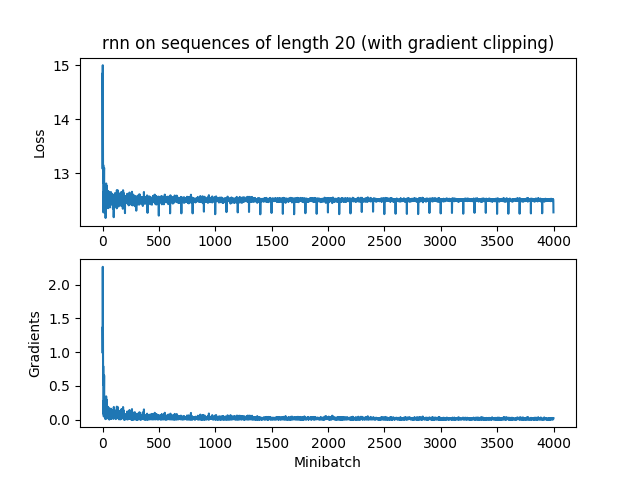
\includegraphics[width=80mm]{assignment3/q3-clip-rnn.png}}
\subfloat[]{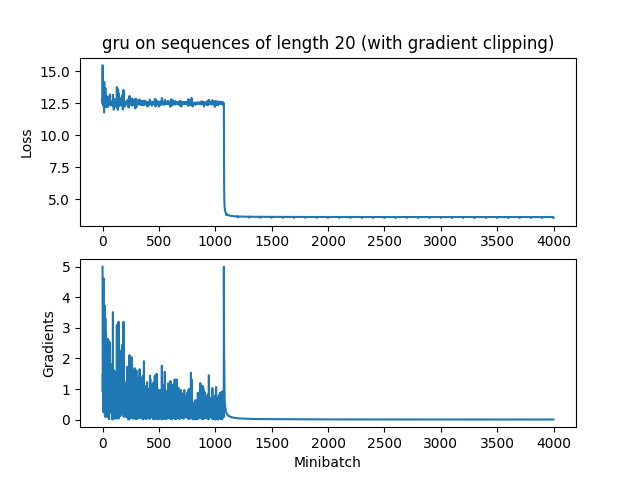
\includegraphics[width=80mm]{assignment3/q3-clip-gru.png}}

\subfloat[]{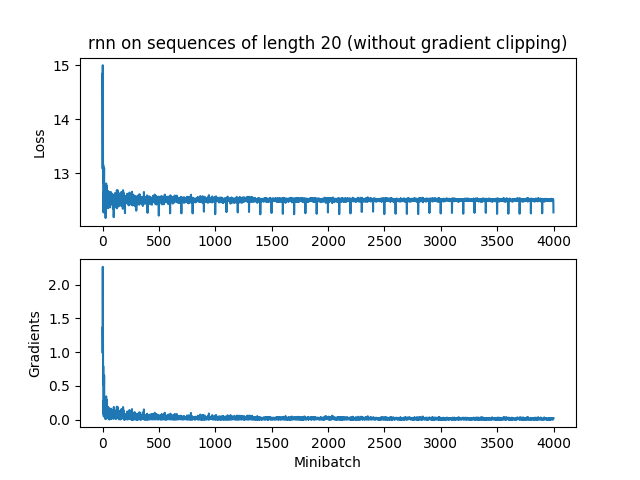
\includegraphics[width=80mm]{assignment3/q3-noclip-rnn.png}}
\subfloat[]{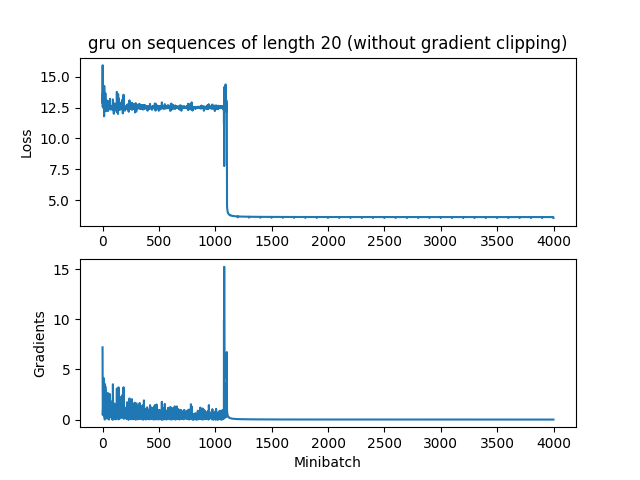
\includegraphics[width=80mm]{assignment3/q3-noclip-gru.png}}
\caption{Gradients and losses from the RNN/GRU experiments with and without gradient clipping.} \label{fig1}
\end{figure}

The results of the experiment are shown in Figure \ref{fig1}.

(e)

\begin{itemize}
\item (i) It seems like all models experienced vanishing gradients. The non-clipped GRU model had a few somewhat large gradients (maximum norm around 15), but nothing that would warrant a description of ``exploding." Since there were no exploding gradients, gradient clipping was not very helpful.
\item (ii) Clipped models and unclipped models performed similarly. The GRUs performed better than the RNNs, probably because they were better able to maintain memory throughout the sequence - you can see that the RNNs quickly entered a state where all the gradients vanished, while the GRUs kept significant gradients through many more training examples.
\end{itemize}
\end{document}
